% v2-acmtog-sample.tex, dated March 7 2012
% This is a sample file for ACM Transactions on Graphics
%
% Compilation using 'acmtog.cls' - version 1.2 (March 2012), Aptara Inc.
% (c) 2010 Association for Computing Machinery (ACM)
%
% Questions/Suggestions/Feedback should be addressed to => "acmtexsupport@aptaracorp.com".
% Users can also go through the FAQs available on the journal's submission webpage.
%
% Steps to compile: latex, bibtex, latex latex
%
% For tracking purposes => this is v1.2 - March 2012
\documentclass{sig-alternate} % V1.2

%\acmVolume{VV}
%\acmNumber{N}
%\acmYear{YYYY}
%\acmMonth{Month}
%\acmArticleNum{XXX}
%\acmdoi{10.1145/XXXXXXX.YYYYYYY}
\usepackage{graphicx}

\begin{document}

\makeatletter
\def\@copyrightspace{\relax}
\makeatother

\title{GLL parsing for embeded languages} % title

\author{Ragozina Anastasiya \\ 
\affil{Saint Petersburg State University}
}
% NOTE! Affiliations placed here should be for the institution where the
%       BULK of the research was done. If the author has gone to a new
%       institution, before publication, the (above) affiliation should NOT be changed.
%       The authors 'current' address may be given in the "Author's addresses:" block (below).
%       So for example, Mr. Fogarty, the bulk of the research was done at UIUC, and he is
%       currently affiliated with NASA.
%}


\maketitle


String-embedded languages are used to generate SQL-queries, HTML-pages, and etc., but ORM technologies are becoming more common and replacing dynamically generated character strings. In spite of this, embedded languages previously were very popular. Now, over the years, it may be necessary to re-engineer such systems. Also this approach is still used in the applications in which performance is crucial. Thus such software needs to be supported in IDE’s (syntax highlighting, autocompletion, error detection) to simplify development process. It is necessary to parse embedded expressions to solve the problems described above. Parsing or syntactic analysis of string-embedded languages allows to check these expressions for errors statically, translate, support in IDEs. 

Unlike host languages, dynamically generated code often cannot be represented as a linear stream, because such
code is usually formed by string operations in loops or conditional statements. To represent nonlinear input we
construct regular over-approximation of possible values for string expressions \cite{Fang Yu}. It
means that instead of linear stream of tokens, a regular set of strings (which can be infinite) is to be
analyzed. Such input can be represented with a finite state automaton which represents all possible values for
string expression. The scheme of the approach is shown in Figure 1. Arithmetic expressions embedded to C\# are
considered as an example. Firstly, it is necessary to get the structural representation of source code written
in C\# (see Figure 1a). This step is carried out by a third-party tool. After that, we construct the automaton
using the structural representation mentioned above. The finite state automaton is represented by a graph with
edges labeled by strings (see Figure 1b). Its graph is an input for the lexer which builds an automaton over
the alphabet of tokens (see Figure 1c). After determinization, the automaton is processed by the parser based
on Generalised LL algorithm (GLL) \cite{GLL}. \textit{Generalised} stands for the property of the algorithm to parse all
context free grammars (including left recursion) and builds parse forest. The parser represent the complete set of derivation trees with a shared packed parse forest (SPPF) \cite{SPPF} in Figure 1d. In SPPF, common subtrees are shared and nodes which correspond to different derivations of the same substring from the same nonterminal are combined. It
allows to reduce the memory required for the parse forest. The red-colored nodes indicate different
subtrees under this nonterminal node. The reasons of this situation are ambiguities in grammar or input. It is
important that this representation is finite even for infinite input (automaton with cycles represent potentially 
infinite input). 

GLL algorithm was chosen because it allows to process ambiguous grammars and reduces the memory required for parsing
by means of using special data structures for stack (GSS) and parse forest (SPPF). Moreover, descriptors which are at the
heart of the GLL technique allow to process nonlinear input with almost no changes in the parsing process. Descriptors
contain the necessary information to re-starts parsing process from the point recorded in the descriptor. Rather than
process single token from the input stream, it covers all outgoing edges from the current node in the input automaton.
Situation when input graph contains cycles is covered too. This is possible due to the fact that the descriptors are
added only once and using of SPPF allows to reuse subtrees and create cycles in them.

Described approach was implemented as a part of the tool YaccConstructor on .NET platform. Figure 1 illustrates the
scheme and results of the parsing algorithm proposed. Current work is the algorithm implementation in Iguana project.
Iguana is a Java implementation of the GLL parsing algorithm with more effective stack \cite{GLL2}. Earlier, as a part of
YaccConstructor project, we proposed and implemented RNGLR-based algorithm for parsing of regular sets. Completeness and
correctness were proved for this algorithm \cite{RNGLR}. Current goal is to compare and unify these approaches.

% Bibliography
\bibliographystyle{ACM-Reference-Format-Journals}
%% PAPEERIA-TEMPLATE\bibliography'{'{1}'}'
                                % Sample .bib file with references that match those in
                                % the 'Specifications Document (V1.5)' as well containing
                                % 'legacy' bibs and bibs with 'alternate codings'.
                                % Gerry Murray - March 2012
\begin{thebibliography}{9}
\bibitem{Fang Yu} Fang Yu, Muath Alkhalaf, Tevfik Bultan, and Oscar H. Ibarra. 2014. Automata-based symbolic string analysis for vulnerability detection. Form. Methods Syst. Des. 44, 1 (February 2014), 44-70. 

\bibitem{GLL} Elizabeth Scott and Adrian Johnstone. 2010. GLL Parsing. Electron. Notes Theor. Comput. Sci. 253, 7 (September 2010), 177-189.

\bibitem{SPPF} Jan Rekers. 1992. Parser generation for interactive environments. Ph.D. thesis, University of Amsterdam.

\bibitem{GLL2} Ali Afroozeh and Anastasia Izmaylova. 2015. Faster, Practical GLL Parsing. Lecture Notes in Computer Science Volume 9031, 89-108

\bibitem{RNGLR} Ekaterina Verbitskaia, Semyon Grigorev, and Dmitry Avdyukhin. 2015. Relaxed Parsing of Regular Approximations of String-Embedded Languages. Unpublished.

\end{thebibliography}

\begin{figure*}[t]
\centering
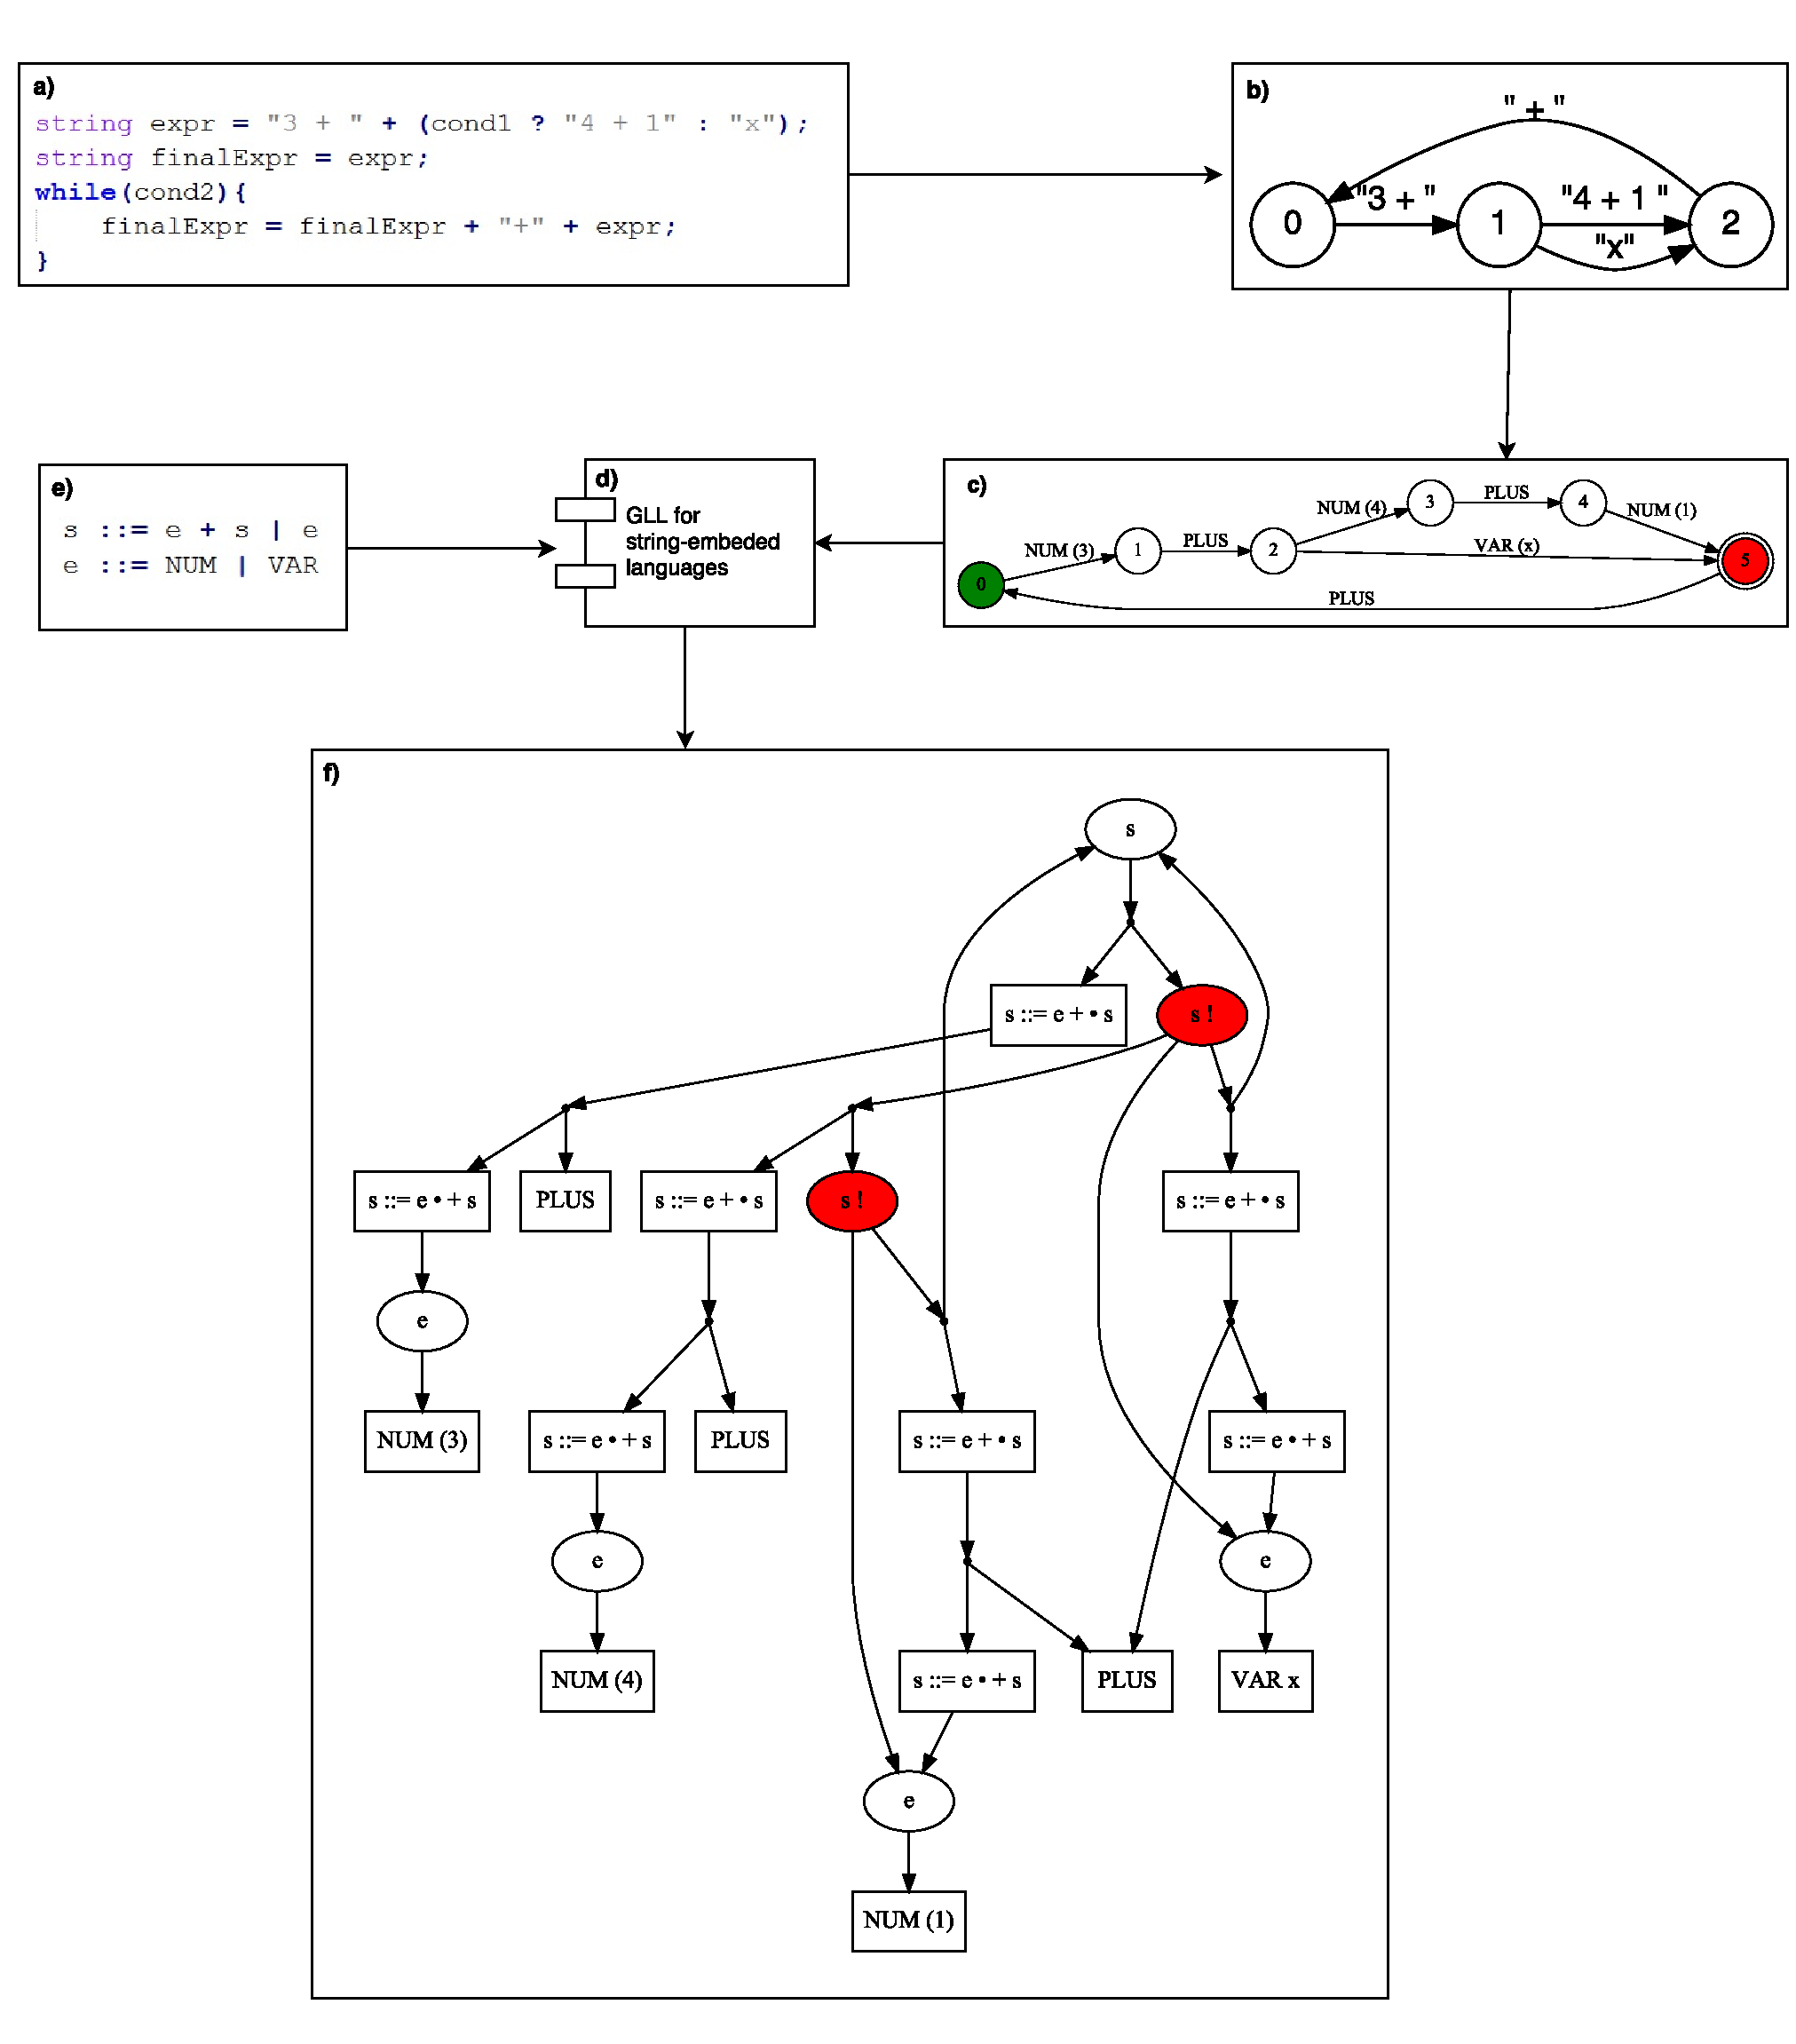
\includegraphics[width=17cm]{pic}
\caption{Scheme of embedded parsing with GLL-based algorithm}
  \label{fig:videocomparison}
\end{figure*}




\end{document}
% End of v2-acmtog-sample.tex (March 2012) - Gerry Murray, ACM
